\begin{figure}[htbp]
\begin{center}
\begin{bigbox}
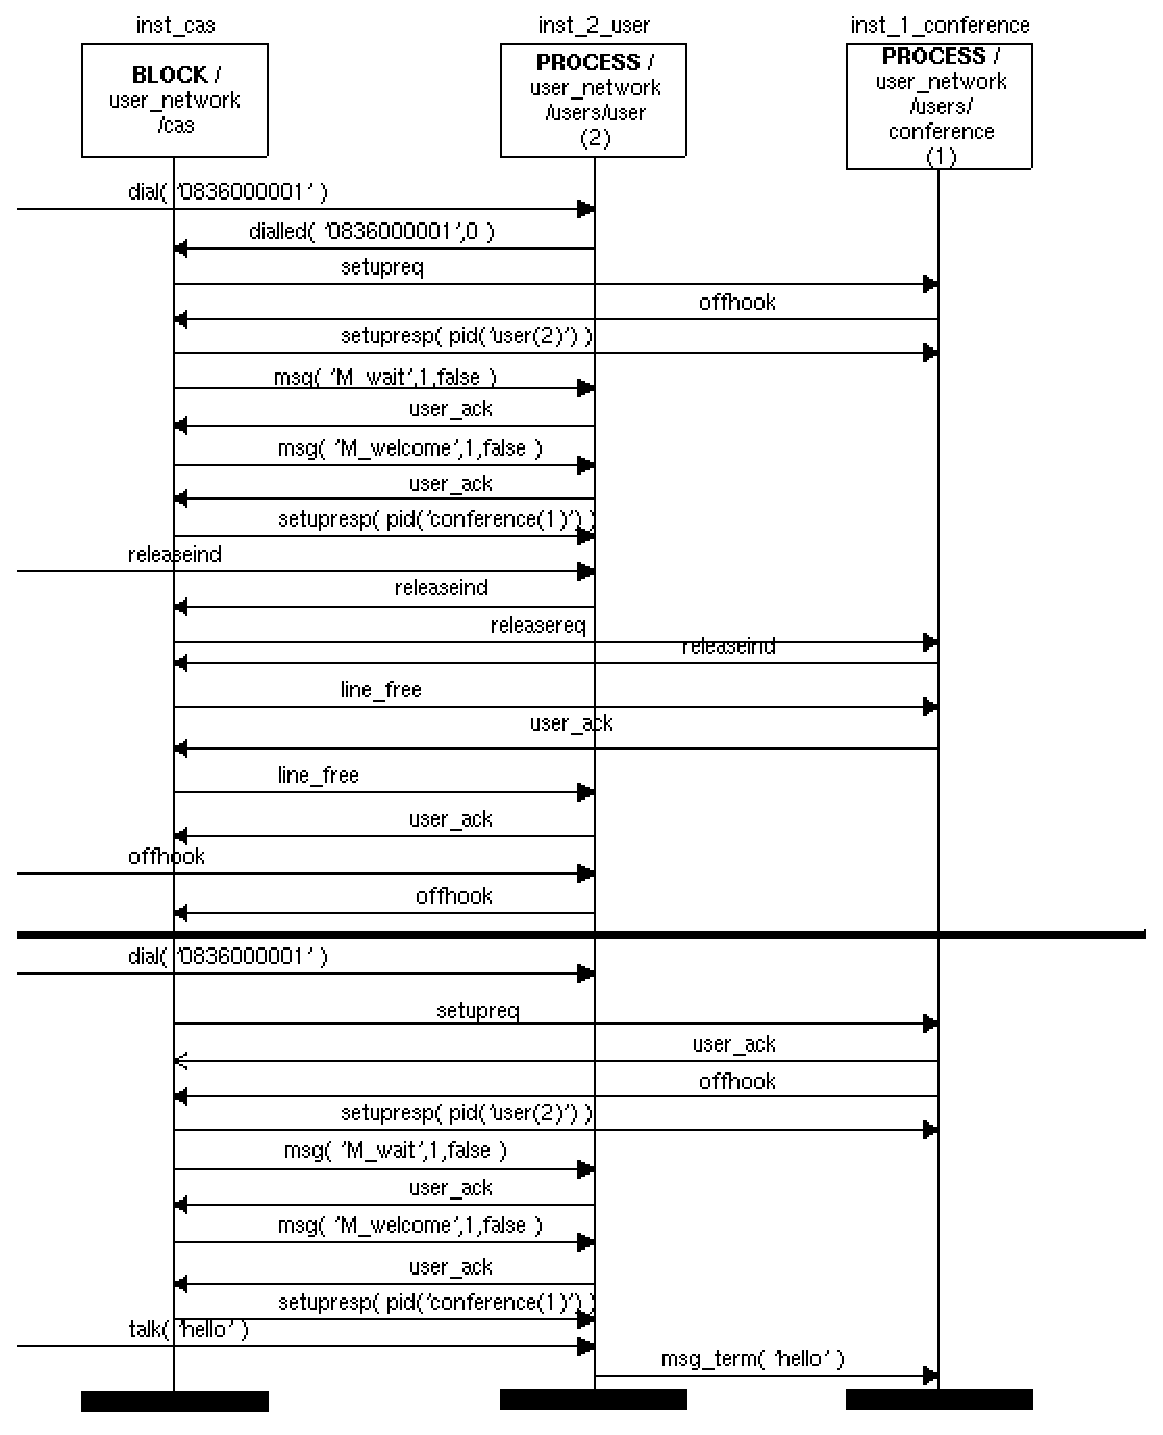
\epsfig{file=msc_final.ps, width=10cm}
\end{bigbox}
\caption{Simplified test sequence of the conference-bridge module.}
\label{msc}
\end{center}
\end{figure}

Figure~\ref{msc} is the simplified MSC for the test sequence obtained
for the module representing the bridge-conference terminal. This
sequence brings to light all the interactions of this module (it
indeed covers all the transitions). We only show here the signal
exchanges between the two peers, i.e. the switch (SSF) and the user,
with which the bridge interacts. The environment here is schematized
by the frame of the figure. The scenarios that can be found in the
signal exchanges of the figure~\ref{msc} are the following:

\begin{itemize}
  \item the user 2 asks for a connection to the \audio by dialing
        number '083600001'. At the conference level, this is
        translated into the signal input \textsf{setupreq}. The
        conference module sends an \textsf{offhook} signal to the
        switch. This latter, after a chaining of exchanges with the PCS
        and a series of component activations, sends a
        \textsf{setupresp} signal which means that the communication
        can be established. First, the user receives a waiting
        message and, as soon as the communication is established, a
        welcome message. Once this latter is received, the user
        decides to on-hook: this sends a \textsf{releaseind} signal to
        the switch; this latter relays it to the conference module by
        means of the \textsf{releasereq}. This latter module
        acknowledges the disconnection request by the
        \textsf{releaseind} signal; then it receives a
        \textsf{line\_free} message, which indicates that the line is
        free again;

  \item the second part of the figure brings to the fore the following
        scenario: the user 1 calls the bridge, he receives the
        waiting signal and then the conference is opened; the waiting
        subscribers receive the welcome message; consequently the
        communication is established, they can talk to each other:
        this exchange is revealed by the reception of a
        \textsf{msg\_term} signal.
\end{itemize}

%We also supply the reader with a part of the TTCN  we got (see
%figure~\ref{ttcnseq}). The computed sequence corresponds to a
%black-box testing configuration, where the points of control and
%observation are located at the system level. Thus the exchanges
%between the environment and the user's block are visible.
%
%\begin{figure*}[!htbp]
%\begin{center}
%\begin{tabular}{l l}
%{\sf Test Case Name} &{\sf: network\_RI\_0}\\
%{\sf Group} &{\sf: network\_RI/}\\
%{\sf Purpose} &{\sf:}\\
%{\sf Default} &{\sf: DEF\_0}\\
%{\sf Comments} &{\sf: Generated by test oriented simulation of the test} \\
%&{\sf \- purpose network\_RI.msc}\\
%\end{tabular}
%\newline
%\scriptsize{
%\begin{tabular}{|p{5mm}|p{75mm}|p{15mm}|p{7mm}|}
%\hline
%{\sf Nr} &{\sf Behaviour Description} & {\sf Constraints Ref}&Verdict\\
%\hline
%{\sf 1} &{\sf env2users !offhook output} &&\\
%{\sf 2} &{\sf \hspace{0.1in}env2users !dial START TAC} & {\sf dial}&\\
%{\sf 3} &{\sf \hspace{0.2in}users ?msg CANCEL TAC} & {\sf msg\_3}&\\ 
%{\sf 4} &{\sf \hspace{0.3in}env2users !dial} & {\sf dial\_4}&\\
%{\sf 5} &{\sf \hspace{0.4in}env2users !releaseind} &&\\
%{\sf 6} &{\sf \hspace{0.5in}env2users !offhook} &&\\
%{\sf 7} &{\sf \hspace{0.6in}env2users !dial START TAC} & {\sf dial\_2}&\\
%{\sf 8} &{\sf \hspace{0.7in}env2users ?msg CANCEL TAC} & {\sf msg\_3}&\\
%{\sf 9} &{\sf \hspace{0.8in}env2users !dial} & {\sf dial\_4}&\\
%{\sf 10} &{\sf \hspace{0.9in}env2users !talk} & {\sf talk\_6}&\\
%{\sf 11} &{\sf \hspace{1.0in}env2users !offhook} &&\\
%{\sf 12} &{\sf \hspace{1.1in}env2users !dial START TAC} & {\sf dial\_7}&\\
%{\sf 13} &{\sf \hspace{1.2in}env2users ?msg CANCEL TAC} & {\sf msg\_3}&\\
%{\sf 14} &{\sf \hspace{1.3in}env2users !dial START} & {\sf dial\_7}&\\
%{\sf 15} &{\sf \hspace{1.4in}env2users ?msg CANCEL} & {\sf msg\_3}&(P)\\
%{\sf 16} &{\sf \hspace{1.4in} ? TIMEOUT TAC} &&F\\
%{\sf 17} &{\sf \hspace{1.2in} ? TIMEOUT TAC} &&F\\
%{\sf 18} &{\sf \hspace{0.6in} ? TIMEOUT TAC} &&F\\
%{\sf 19} &{\sf \hspace{0.1in} ? TIMEOUT TAC} &&F\\
%\hline
%\end{tabular}
%}
%\caption{TTCN sequence}
%\label{ttcnseq}
%\end{center}
%\end{figure*}
